\section{Einleitung}
	\label{sec:einleitung}
	In diesem Versuch soll der Wirkungsgrad einer Solarzelle bestimmt werden.
	Durch Messung von Strom und Spannung und mit Kenntniss der Intensit"at des einfallenden Lichtes l"asst sich dieser bestimmen.


\section{Theorie und Hintergrund}
	\label{sec:theorie}

	\subsection{Aufbau und Funktion einer Solarzelle}
		\label{subsec:aufbau_funktion}
		Eine Solarzelle ist grunds"atzlich aufgebaut wie eine Diode.
		Eine p- und n-dotierte Halbleiterschicht werden zusammengebracht, wodurch am Grenzbereich ein starkes elektrisches Feld entsteht.

		Im Folgenden soll dies etwas erl"autert werden.

		\subsubsection{Halbleiter}
			\label{subsub:halbleiter}
			Festk"orper k"onnen anhand ihrer elektrischen Leitf"ahigkeit in drei Kategorien eingeteilt werden.
			Neben Leitern, in denen sich Elektronen nahezu frei bewegen k"onnen, gibt es Isolatoren, in denen Elektronen sehr viel Energie ben"otigen, um sich vom Atomkern zu l"osen.
			In Halbleiter dagegen k"onnen Elektronen unter bestimmten Umst"anden gebunden sein oder leicht von ihrem Kern getrennt werden.

			
			Dieses Ph"anomen kann man mit dem B"andermodell beschreiben.
			Die Elektronen in einem Festk"orper besitzen verschiedene Energieniveaus.
			W"ahrend ein Elektron eines einzelnen Atoms nur diskrete Energien besitzen kann, erweitern sich diese Niveaus in einem Festk"orper zu Energieb"andern mit kontinuierlichen Dimensionen.
			In dieser Betrachtung besitzt jeder Festk"orper zwei charakteristische B"ander.

			Zum einen das Valenzband, welches den Bereich beschreibt, in dem sich die Elektronen mit der gr"o"sten Energie befinden, die jedoch noch an den Atomkern gebunden sind.
			Energetisch h"oher liegt das Leitungsband.
			Elektronen die so viel Energie besitzen, dass sie sich in diesem Bereich aufhalten, k"onnen sich frei durch den K"orper bewegen.
			
			\begin{figure}[h!]
				\centering
				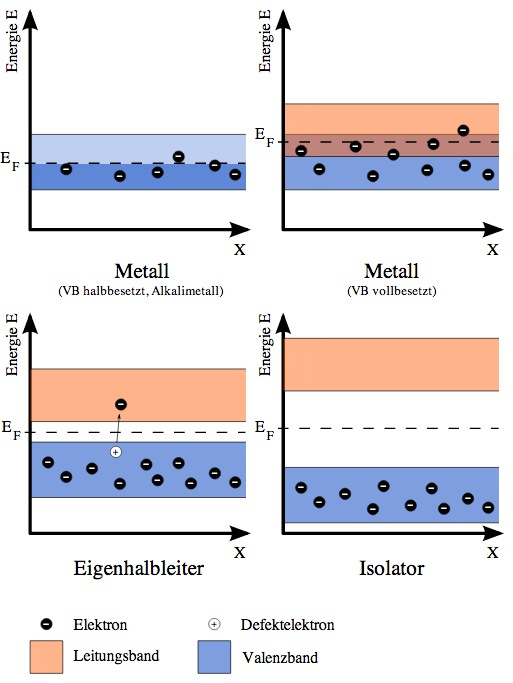
\includegraphics[width = 8cm]{img/baender.JPG}
				\caption{Das B"andermodell schematisch dargestellt \cite{wiki}}
				\label{fig:baendermodell}
			\end{figure}

			In Leitern "uberschneiden sich Beide Bereiche.
			Selbst unangeregte Elektronen befinden sich im Leitungsband.
			Das Material kann elektrisches Strom somit ohne weiteres Leiten.

			Isolatoren zeichnen sich dadurch aus, dass der Abstand zwischen beiden B"andern so gro"s ist, dass die Elektronen praktisch nicht in der Lage sind ihn zu "uberwinden.
			Sie sind somit stets an den Kern gebunden und das Material leitet keinen elektrischen Strom.

			In Halbleitern ist der B"anderabstand dagegen so klein, dass er mit geringer Anregung der Elektronen "uberwunden werden kann und das Material dann Leitend wird.
			Das angeregte Elektron hinterl"asst im Valenzband eine L"ucke, die durch nachr"uckende Elektronen gef"ullt wird.
			Das so entstandene Loch wandert durch das Material und tr"agt damit zum Strom bei.
			Es kann als positive Ladung betrachtet werden.

		\subsubsection{Dotierung von Halbleitern und "Uberg"ange}
			\label{subsub:dotierung}
			Es k"onnen Fremdatome in ein Halbleitermaterial gebracht werden, die mehr oder weniger Elektronen im Valenzband haben, als der Halbleiter selbst.
			Dadurch verschiebt man die B"ander zueinander.
			Wird das Valenzband angehoben, spricht man von n-dotierten Halbleitern.
			Im Gegensatz dazu hei"sen Halbleiter mit verringertem Leitungsband p-dotiert.


			Bringt man nun n- und p-dotierte Halbleiter in Kontakt, flie"sen die "ubersch"ussigen Elektronen aus dem n-Halbleiter zum p-Halbleiter und rekombinieren mit den dortigen L"ochern.
			Weil nun die verschieden dotierten Festk"orper unterschiedliche Elektronendichten aufweisen, ensteht im Grenzbereich zwischen ihnen ein elektrisches Feld.
			Diesen Bereich nennt man Raumladungszone.

		\subsubsection{Ladungstrennung und Strom}
			\label{subsub:ladungstrennung}
			Photonen mit gen"ugend Energie sind in der Lage, Elektronen anzuregen und aus ihrer Atomh"ulle zu entfernen.
			Trifft Sonnenlicht auf die oben beschrieben Raumladungszone einer Solarzelle, besteht die M"oglichkeit, dass in genau diesem Bereich ein Elektron von seinem Atom getrennt wird.
			Das elektrische Feld "ubt nun eine gen"ugend gro"se Kraft auf das Elektron aus, damit es sich von seinem Kern entfernt und in den Halbleiter abgef"uhrt wird.
			Gleichzeitig ensteht ein Loch, welches in entgegengesetzer Richtung abgelenkt wird.

			Werden beide Halbleiter au"senseitig miteinander Verbunden, kann das Elektron-Loch Paar "uber einen Verbraucher abflie"sen und rekombinieren.
			Der so entstehende Strom kann Arbeit verrichten.

		\begin{figure}[h]
			\centering
			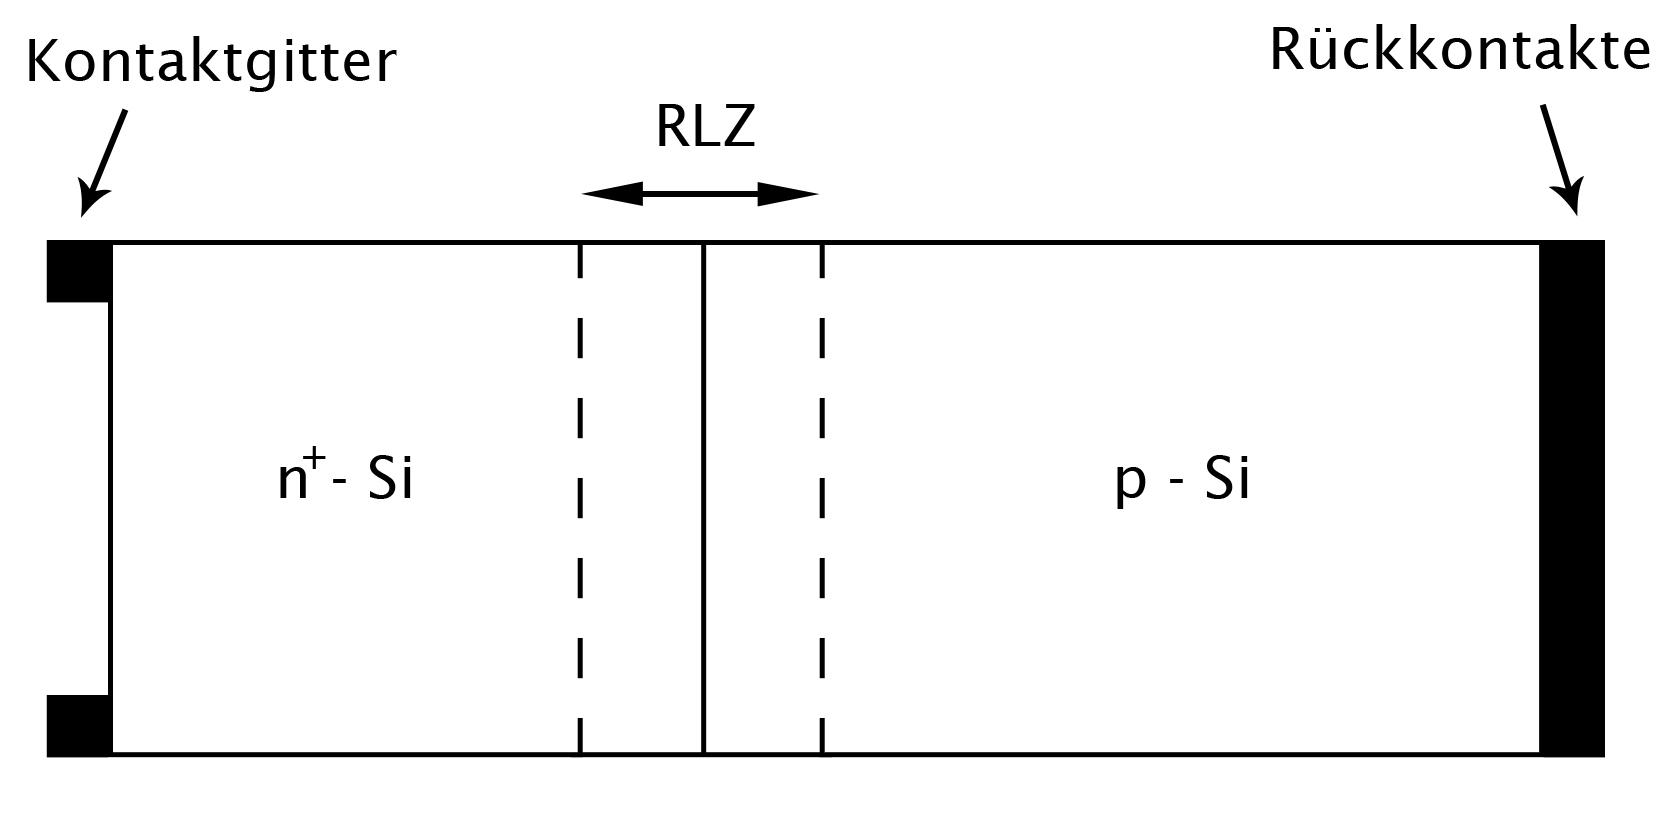
\includegraphics[width = 15cm]{img/diode_neu.jpg}
			\caption{Schematischer Aufbau einer Solarzelle}
			\label{fig:diode}
		\end{figure}

	\subsection{Technische Umsetzung}
		\label{sub:umsetzung}
		Als Rohstoff f"ur die meisten Solarzellen dient Silizium.
		Es kann g"unstig verarbeitet werden und der Umgang mit diesem Stoff ist gut erforscht.
		Nachdem in den letzten Jahrenzehnten zun"achst monokristallines und sp"ater multikristallines Silizium (c-Si) verwendet wurde,
		versucht man heute, die Effizienz von amorphen Silizium (a-Si) zu erh"ohnen, um dieses marktf"ahig zu machen.

		Bei c-Si geht w"ahrend der Herstellung der Wafer n"amlich viel Material verloren, was die Kosten steigen l"asst.
		Wafer aus a-Si k"onnen dagegen nahezu verlustfrei hergestellt werden.
		Der Wirkungsgrad $\eta$ von a-Si ist jedoch noch zu gering um es wirtschaftlich nutzen zu k"onnen.

	\subsection{Berechnung des Wirkungsgrades $\eta$}
		\label{subsec:wirkungsgrad}
		F"ur den Wirkungsgrad $\eta$ der Zelle ist das Verh"altnis aus entnommener Leistung $P_\mathrm{max}$ und einfallender Leistung $P_\mathrm{ein}$ entscheidend.

		Es gilt

		\begin{equation}
			\eta = \frac{P_\mathrm{max}}{P_\mathrm{ein}} = \frac{U_\mathrm{o} I_\mathrm{k} F}{P_\mathrm{ein}} .
		\end{equation}

		Hier bezeichnet $U_\mathrm{o}$ die Spannung bei offenem Stromkreis und $I_\mathrm{k}$ den Kurzschlussstrom. Der F"ullfaktor $F$ bezeichnet das Verh"altnis der maximalen Fl"ache unter der I-U-Kennlinie zur Fl"ache $I_\mathrm{k} \cdot U_\mathrm{o}$.